\documentclass[11pt]{article}
\usepackage{amsmath}
\usepackage{caption}

\usepackage{algorithmicx}
\usepackage{verbatim}
\usepackage{algpseudocode}
\usepackage{algorithm}
\setlength{\parindent}{0pt}

\usepackage{graphicx}
\usepackage{listings}

\title{Exercisesheet No.4}
\author{Alexander Diete \and Magnus M\"uller \and Martin Pfannem\"uller}

\begin{document}
\maketitle

\section*{Ex.1}
a) Only network ii) and iii) can represent the problem correctly. Network i) does not have a connection between Wrapper and Shape. Since the probability of the shape is not independent from the wrapper (and vice versa) this network cannot represent the given problem. \\

b) Network number iii) is the best choice as it correctly represents the problem. Also it is simpler than the network ii) which shows an implication from the wrapper to shape. \\

c) Yes as it does not show any connection between the wrapper and the shape. This implies that the two events are independent from each other. Hence this would mean the conditional probability P(wrapper|shape) is equal to P(wrapper). \\

d) 
$$P(strawberry) \cdot P(red|strawberry) + P(anchovy) \cdot P(red|anchovy)$$
$$0.7 \cdot 0.8 + 0.3 \cdot 0.1 = 0.59$$ \\

e)
$$\frac{P(strawberry | red, round)}{P(strawberry | red, round) + P(anchovy | red, round)}$$
$$\frac{0.7 \cdot 0.8 \cdot 0.8}{0.7 \cdot 0.8 \cdot 0.8 + 0.3 \cdot 0.1 \cdot 0.1} = \frac{0.448}{0.451} \approx 0.993$$ \\

\section*{Ex.2}
Given the following probabilities and their payoffs:\\
\begin{tabular}{|l|c|c|}
\hline
    A & 80\% & \$4000 \\
    \hline
    B & 100\% & \$3000 \\
    \hline
    C & 20\% & \$4000 \\
    \hline
    D & 25\% & \$3000 \\
    \hline
\end{tabular}
\\
It follows by decomposability that: $C\sim[25\%,A; 75\%,0]$ and $D\sim[25\%,B;75\%,0]$. \\
By substitutability that: if $D \prec C$ then we $B \prec A$ would have to hold. This leads to a contradiction with respect to the assumption $D \prec C$ and $A \prec B$.
\section*{Ex.3}
a) \\
\begin{figure}[ht]
	\centering
  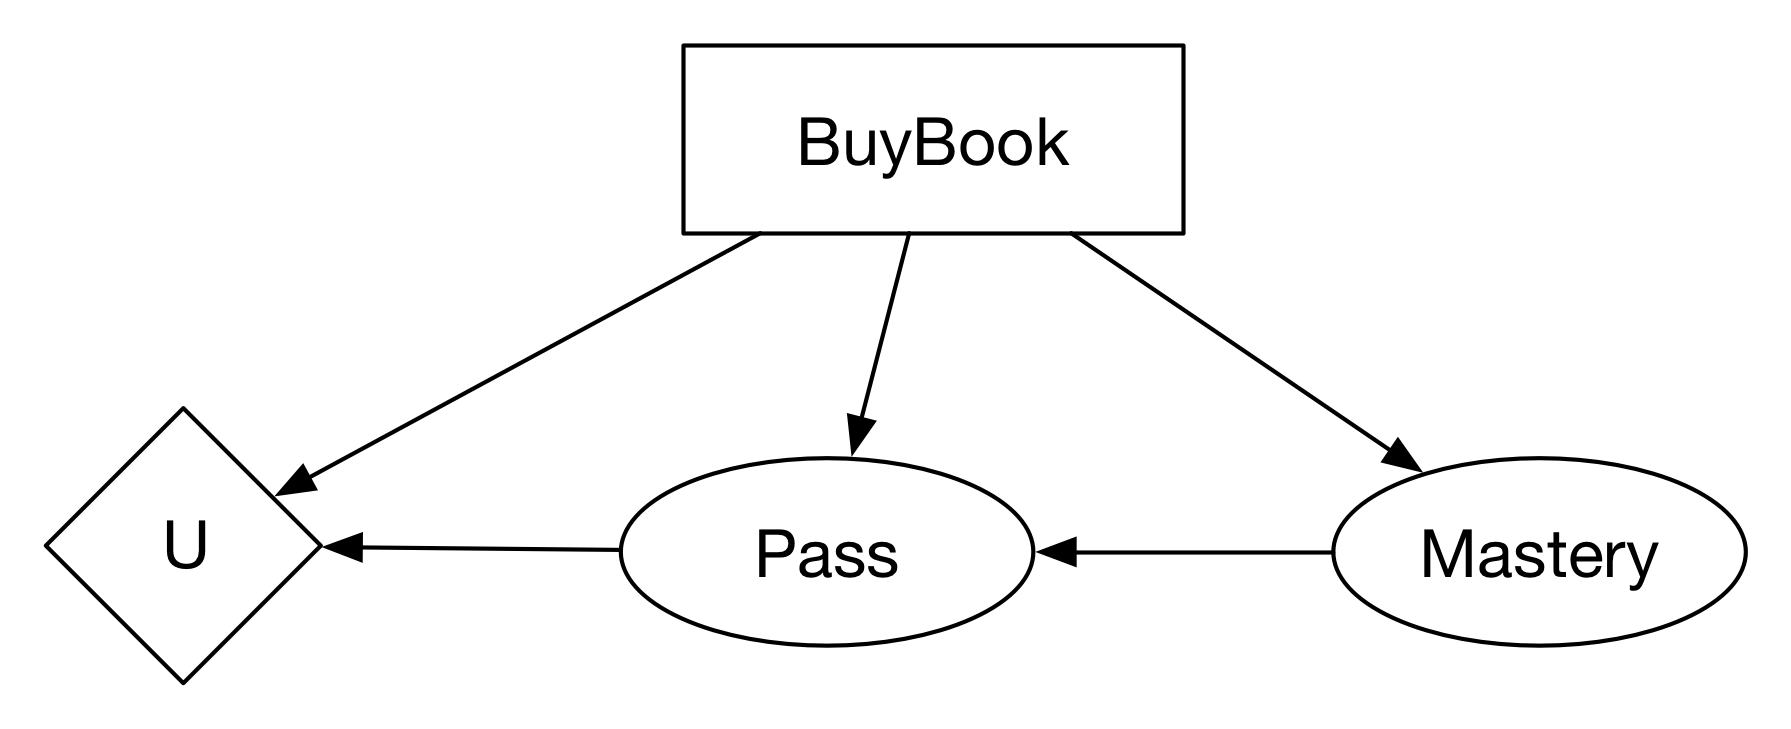
\includegraphics[width=0.7\textwidth]{DecisionNetwork}
	\caption{Ex.3a}
	\label{fig:3}
\end{figure}
\\
b) Utility of buying the book: \\ \\
$(P(p|b,m) \cdot P(m|b) + P(p|b\neg m) \cdot P(\neg m|b)) \cdot (2000-100)\$ + $

$(P(\neg p|b, m) \cdot P(m|b) + P(\neg p|b,\neg m) \cdot P(\neg m|b)) \cdot -100\$$

$$(0.9 \cdot 0.9 + 0.5 \cdot 0.1) \cdot (2000-100)\$ +  (0.1 \cdot 0.9 + 0.5 \cdot 0.1) \cdot -100\$ = 1.706\$ $$

Utility of not buying the book:
$$(P(p|\neg b,m) \cdot P(m|\neg b) + P(p|\neg b, \neg m) \cdot P(\neg m|\neg b)) \cdot 2000\$ $$
$$ (0.8 \cdot 0.7 + 0.3 \cdot 0.3) \cdot 2000\$ = 1300\$$$

c) Sam should buy the book. 
\end{document}